\documentclass[12pt,titlepage,bibliography=totoc]{article}
\usepackage[utf8]{inputenc}
\usepackage[T1]{fontenc}
\usepackage[english]{babel}
\usepackage[a4paper]{geometry}
\frenchspacing
\usepackage{amsfonts}
\usepackage{amsmath}
\usepackage{amssymb}
\usepackage{amsthm}
\usepackage{setspace}
\usepackage{fullpage}
\usepackage{tocbibind}
\usepackage{graphicx}
\usepackage{url}
\usepackage{verbatim}
\usepackage{listings}
%\usepackage{gitinfo2}
\usepackage{hyperref}
\usepackage{cleveref}
\usepackage{cite}
\usepackage{color}
\usepackage{enumitem}
\usepackage{usecases}
\usepackage{nameref}

\definecolor{pblue}{rgb}{0.13,0.13,1}
\definecolor{pgreen}{rgb}{0,0.5,0}
\definecolor{pred}{rgb}{0.9,0,0}
\definecolor{pgrey}{rgb}{0.46,0.45,0.48}
\lstset{language=Java,
  showspaces=false,
  showtabs=false,
  breaklines=true,
  showstringspaces=false,
  breakatwhitespace=true,
  commentstyle=\color{pgreen},
  keywordstyle=\color{pblue},
  stringstyle=\color{pred},
  basicstyle=\ttfamily,
  moredelim=[il][\textcolor{pgrey}]{$$},
  moredelim=[is][\textcolor{pgrey}]{\%\%}{\%\%}
}
\renewcommand{\labelitemi}{$\bullet$}
\renewcommand{\labelitemii}{$\cdot$}
\renewcommand{\labelitemiii}{$\diamond$}
\renewcommand{\labelitemiv}{$\ast$}


\begin{document}
\title{
	Design Document for Bicycle Garage Pro\\
	(Group 33, 2015)\\
	\vspace{0.2in}
	\normalsize Current version: 0.9.1
}
\author{
	Alexander Skafte\\
	\url{tfy13ask@student.lu.se}\\
	Dennis Jin\\
	\url{desuvader@gmail.com}\\
	Petter Berntsson\\
	\url{dat14pbe@student.lu.se}\\
	Emelie Löthman\\
	\url{pol14elo@student.lu.se}\\
	Adam Mzrozek\\
	\url{dat14amr@student.lu.se}
}
\date{}



\maketitle
\newpage
\tableofcontents
\thispagestyle{empty}
\setcounter{page}{0}
\newpage

\section{Introduction}
\subsection{Purpose}
This document describes the requirements and functionalities of the \emph{Bicycle Garage Pro} software.

The intended audience of this document are mainly: software developers, in order to aid the development of the software; and clients, in order to provide an accurate overview of the project.

\subsection{Glossary}
Despite this being a software-only specification, relevant hardware-related terms are still explained for convenience's sake.
\begin{enumerate}
	\item General terms
	\begin{enumerate}
		\item BGP - Bicycle Garage Pro (software)
		\item ACME - The company which BGP is produced for
		\item User - A cyclist who uses the Bicycle Garage Pro system
		\item Operator - Subject responsible for managing BGP (on-site)
		\item Entrance - Main entrance door of the garage. Electronic lock.
		\item Exit 1 - Garage exit for users with bicycles. Electronic lock.
		\item Exit 2 - Garage exit for users without bicycles. Can be opened from inside the garage.
	\end{enumerate}

	\item Software-related terms
	\begin{enumerate}
		\item (The) System - Bicycle Garage Pro software
		\item GUI - Graphical user interface
		\item CRUD - Create, read, update and delete (operations)
		\item PIN - 4-digit code, used to access the garage
		\item API - Application programming interface
		\item Database - System-relevant data is store in the database
	\end{enumerate}

	\item Hardware-related terms
	\begin{enumerate}
		\item PC - Personal computer
		\item LED - Light-emitting diode
		\item Barcode reader - Device that can read/scan barcodes
		\item Barcode printer - Device that can print barcodes
		\item PIN terminal - Terminal where a PIN can be entered
		\item Electronic lock - Electronically controlled lock on the entrance and exit 1
	\end{enumerate}
\end{enumerate}

\subsection{Scope}
BGP is a software application that manages a bicycle garage. This requirement specification only covers the software part for the bicycle garage and the following assumptions are therefore made about the hardware:
\begin{enumerate}
	\item The hardware handles recognition and reading (scanning) of barcodes
	\item The hardware handles printing of barcodes
	\item The hardware handles locking and unlocking of doors
	\item The hardware handles reading of PINs
\end{enumerate}
The hardware, as stated above, will be accessed by the system according to a predefined API. See \cref{app:hardware} for a more detailed description of the API.

\subsection{Goals}
\subsubsection{Business goals}
ACME is a company that works in the bicycle garage business in Sweden. ACME aims to provide low-cost, semi-automated bicycle garage solutions for public use. The goals for ACME with this software are mainly:
\begin{enumerate}
	\item Customer retention through maintainability
\end{enumerate}
\subsubsection{Product goals}
The goal of BGP is to assist in managing a bicycle garage by keeping track of users and their bicycles. The user interface should be simple to use and the software should be easily maintainable for future developers.

\subsection{Overview}
The structure of this specification is based on guidelines from the ETSA01 course website and the ETSA01 course compendium \cite{kompendium,course-site}.

\section{Product description}
\label{sec:proddesc}

For clarification purposes, see \cref{fig:garage} for an example on how the complete garage facility (physical) can look like. The PC runs BGP.

The interactions between the system and external entities, that may interact with the system, can be seen in \cref{fig:context-hw}. The control unit is the BGP software. The arrows in \cref{fig:context-hw} mainly aim to specify software-related signals that are relevant to this specification.

\begin{figure}
	\centering
	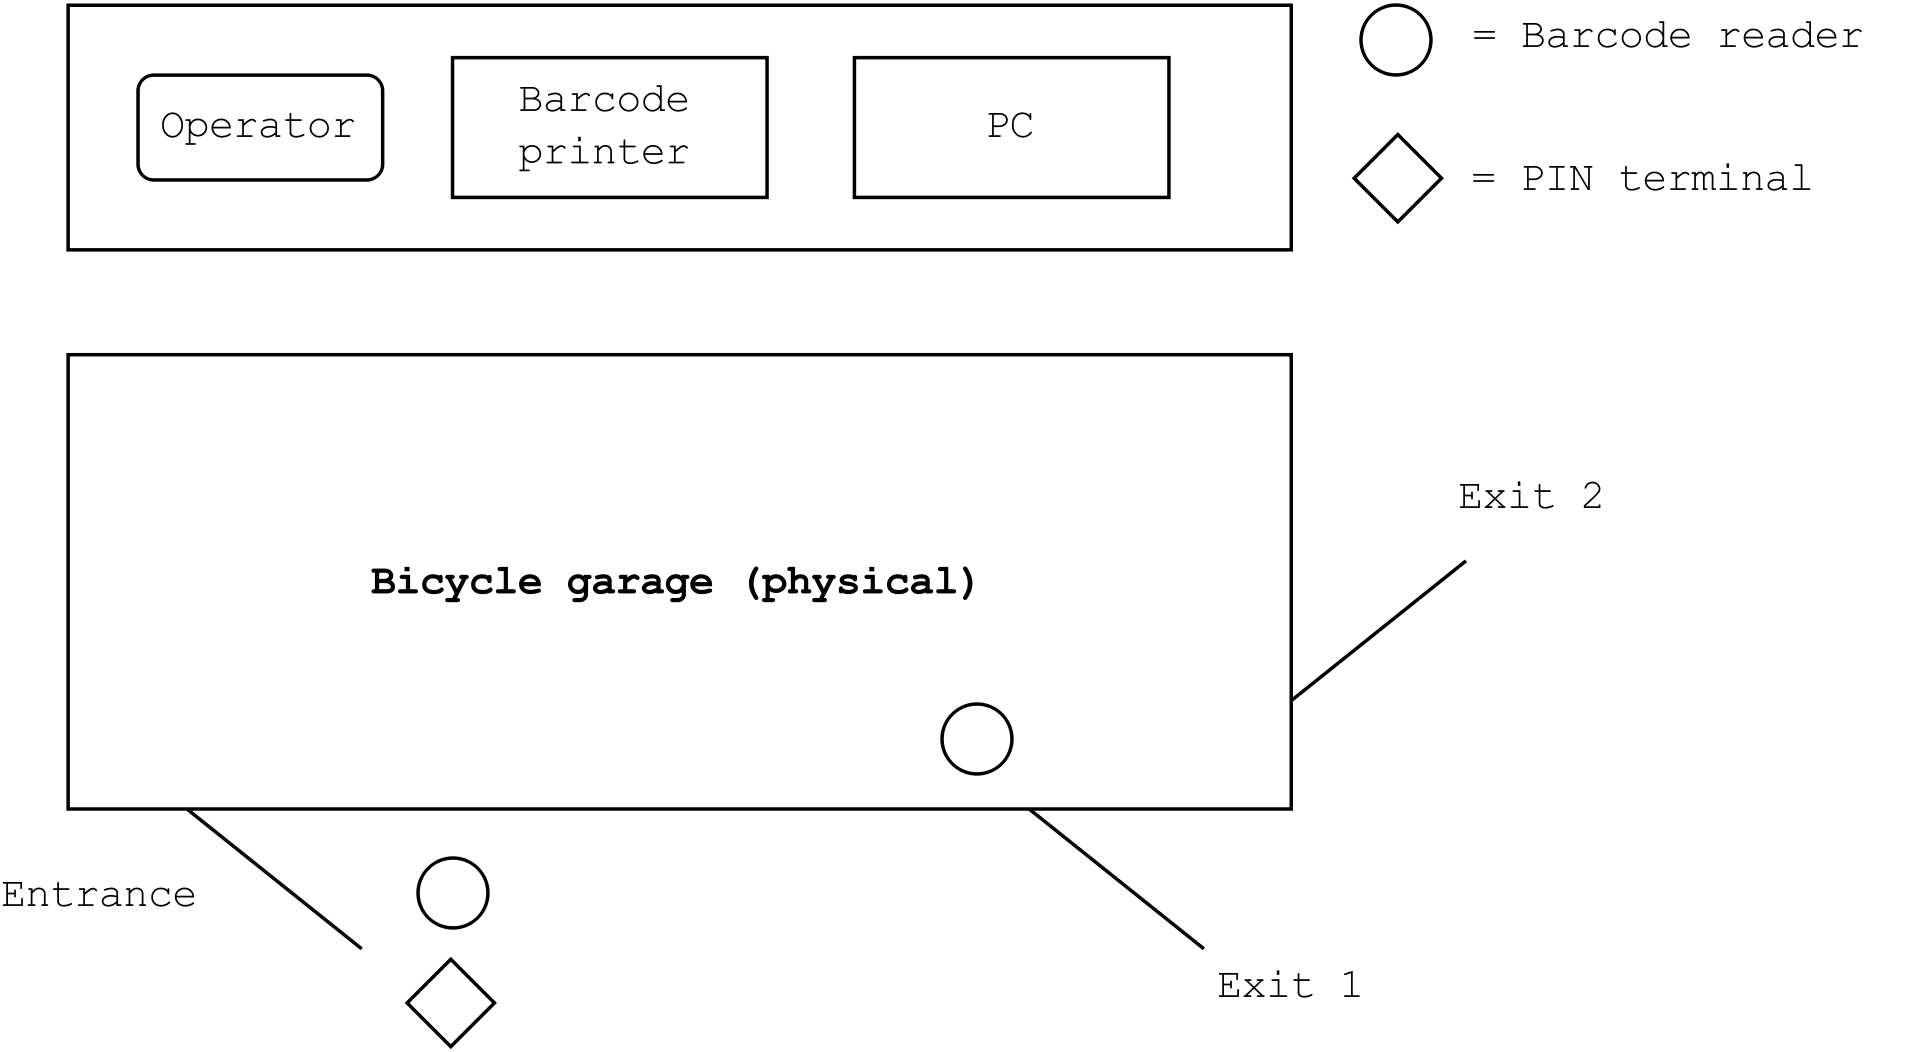
\includegraphics[width=0.9\textwidth]{./assets/garage.png}
	\caption{Simple example of how the complete garage system would look}
	\label{fig:garage}
\end{figure}

\begin{figure}
	\centering
	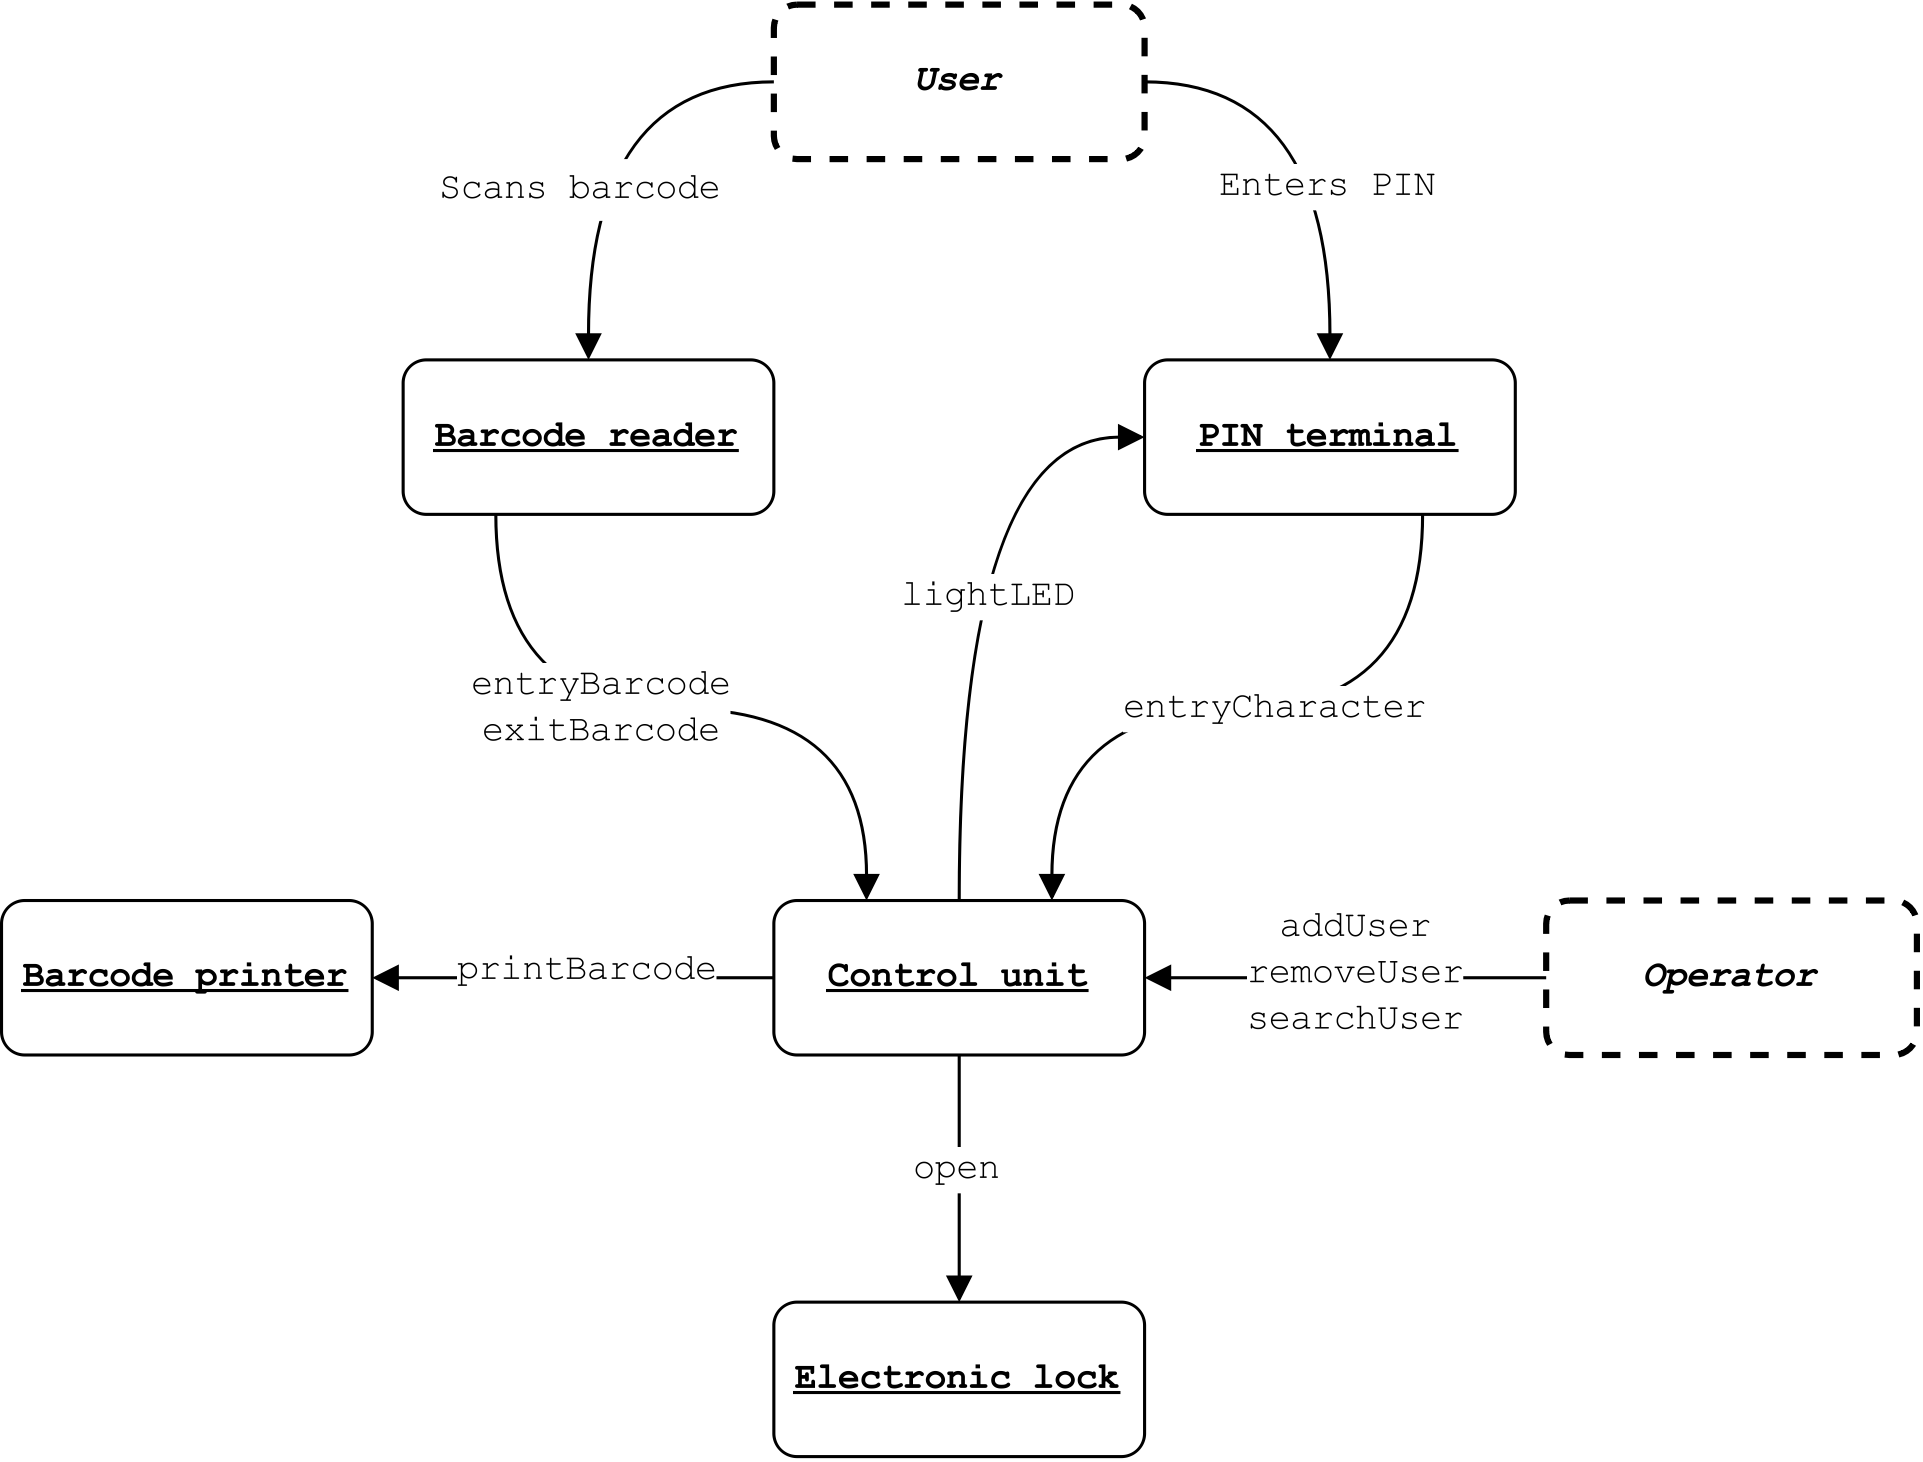
\includegraphics[width=0.9\textwidth]{./assets/context.png}
	\caption{Context diagram for BGP}
	\label{fig:context-hw}
\end{figure}


\begin{enumerate}
	\item The control unit sends out the following signals:
	\begin{enumerate}
		\item lightLED - Sent out depending on success/failure when entering PIN or scanning barcode
		\item printBarcode - Sent out when a barcode should be printed through the barcode printer
		\item open - Sent out to either the entrance or exit 1, and unlocks the door (electronic lock)
	\end{enumerate}
	\item The control unit receives the following signals:
	\begin{enumerate}
		\item entryCharacter - Received when a button is pressed on the PIN terminal
		\item entryBarcode - Received when a barcode is scanned at the entrance
		\item exitBarcode - Received when a barcode is scanned at the exit
		\item addUser - Received when the operator wants to add an user
		\item removeUser - Received when the operator wants to remove an user
		\item getUserByNIN - Received when the operator wants to search for an user by national identification number
	\end{enumerate}
\end{enumerate}

\section{Requirements}
\subsection{Interface}
BGP should support the API defined in \cref{sec:proddesc}.
\subsection{Use cases}
\label{sec:cases}
The use cases below are the most typical scenarios that one would run into when using the bicycle garage. The idea is that the system should at least be able to handle these use cases. Keep in mind that this isn't a complete description of the system and should therefore not be used as the main guidelines for developing the system.

\begin{usecase}
	\addtitle{Use case 1:}{User wants to store a bicycle}
	\addfield{Primary actor:}{User}
	\addfield{Preconditions:}{User is registered.}
	\addfield{Postconditions:}{The bicycle of the user checked in.}
	\addscenario{Main success scenario:}{
		\item User scans their barcode at the entrance.
		\item The entrance door unlocks.
	}
	\addscenario{Exception scenarios:}{
		\item [1.a] Barcode is not recognized:
			\begin{enumerate}
				\item[1.] Use case ends here. The remaining steps are skipped.
			\end{enumerate}
		\item [1.b] Bicycle is already checked in:
			\begin{enumerate}
				\item[1.] Use case ends here. The remaining steps are skipped.
			\end{enumerate}
	}
\end{usecase}

\begin{usecase}
	\addtitle{Use case 2:}{User wants to retrieve a bicycle}
	\addfield{Primary actor:}{User}
	\addfield{Preconditions:}{User is registered. User has a registered bicycle, stored in the garage.}
	\addfield{Postconditions:}{The bicycle of the user is checked out.}
	\addscenario{Main success scenario:}{
		\item User enters their PIN at the entrance.
		\item The entrance door unlocks.
		\item The user scans their barcode at exit 1.
		\item Exit 1 unlocks.
	}
	\addscenario{Exception scenarios:}{
		\item [1.a] PIN is incorrect:
			\begin{enumerate}
				\item[1.] Red LED blinks to indicate failure.
				\item[2.] Use case ends here. The remaining steps are skipped.
			\end{enumerate}
		\item [3.a] Barcode is not recognized:
			\begin{enumerate}
				\item[1.] Use case ends here. The remaining steps are skipped.
			\end{enumerate}
		\item [3.b] Bicycle is already checked out:
			\begin{enumerate}
				\item[1.] Use case ends here. The remaining steps are skipped.
			\end{enumerate}
	}
\end{usecase}

\begin{usecase}
	\addtitle{Use case 3:}{User wants to register}
	\addfield{Primary actor:}{Operator}
	\addfield{Preconditions:}{User is unregistered.}
	\addfield{Postconditions:}{The user, coupled with their bicycle (indentified by barcode), has been added to the system. The user has access to the garage.}
	\addscenario{Main success scenario:}{
		\item Operator adds the user to the system.
		\item Operator provides the user with an unique barcode.
		\item Operator provides the user with a PIN.
	}
\end{usecase}

\begin{usecase}
	\addtitle{Use case 4:}{User wants to unregister}
	\addfield{Primary actor:}{Operator}
	\addfield{Preconditions:}{User is registered.}
	\addfield{Postconditions:}{The user has been removed from the system.}
	\addscenario{Main success scenario:}{
		\item The operator removes the user from the system.
	}
	\addscenario{Exception scenarios:}{
		\item [1.a] User has a checked in bicycle:
			\begin{enumerate}
				\item[1.] User is removed anyways.
				\item[2.] User will have to contact the operator for assistance.
			\end{enumerate}
	}
\end{usecase}

\begin{usecase}
	\addtitle{Use case 4:}{User wants to remember their PIN}
	\addfield{Primary actor:}{Operator}
	\addfield{Preconditions:}{User is registered.}
	\addscenario{Main success scenario:}{
		\item The operator verifies that the user exists in the system.
		\item The operator provides the user with their PIN.
	}
\end{usecase}

\begin{usecase}
	\addtitle{Use case 4:}{User wants to store a bicycle in a full garage.}
	\addfield{Primary actor:}{User}
	\addfield{Preconditions:}{User is registered. Garage is full.}
	\addscenario{Main success scenario:}{
		\item User scans their barcode at the entrance.
		\item Door stays locked because the garage is full.
	}
\end{usecase}
\subsection{Functional requirements}
\subsubsection{User-related requirements}
\begin{enumerate}
	\item The system shall keep track of following about an user:
	\begin{enumerate}
		\item First name and last name
		\item National identification number (unique 10-digit string)
		\item Unique PIN (unique 4-digit integer)
	\end{enumerate}
	\item Each users shall have an unique 4-digit PIN that only consist of numbers ranging from 0 to 9 (inclusive).
	\item The system shall store user data in a database.
	\item The system shall be able to add users to the database.
	\item The system shall be able to remove users from the database.
	\item The system shall be able to search for users in the database, by national identification number.
	\item The system shall not be able to add users once all unique PINs are in use.
	\item When users are removed from the database, the system shall be able to reuse the unique PIN.
\end{enumerate}
\subsubsection{Bicycle-related requirements}
\begin{enumerate}
	\item The system shall keep track of following about a bicycle:
	\begin{enumerate}
		\item Bicycle ID (unique 5-digit integer)
		\item Date of when the bicycles was last checked in
		\item Date of when the bicycles was last checked out
		\item Whether the bicycle is checked-in or not
	\end{enumerate}
	\item The system shall store bicycle data in a database.
	\item The system shall be able to add bicycles to the database.
	\item The system shall be able to remove bicycles from the database.
	\item The system shall not be able to add bicycles once all unique Bicycle IDs are in use.
	\item The system shall not allow more than 500 checked in bicycles, in the garage, at a time.
	\item When bicycles are removed from the database, the system shall be able to reuse the bicycle ID.
\end{enumerate}
\subsubsection{Interaction-related requirements}
\begin{enumerate}
	\item When a \emph{correct} PIN is entered at the entrance:
		\begin{enumerate}
			\item The LED shall show green for 4 seconds.
			\item The system shall unlock the entrance for 10 seconds.
		\end{enumerate}
	\item When an \emph{incorrect} PIN is entered at the entrance the LED shall show red for 4 seconds.
	\item When a recognized barcode is scanned at the entrance:
		\begin{enumerate}
			\item The system shall unlock the entrance for 10 seconds.
			\item A new check-in date should be set for the bicycle.
		\end{enumerate}
	\item When a recognized barcode is scanned at exit 1, the system shall unlock the exit for 10 seconds.
\end{enumerate}
\subsubsection{Miscellaneous}
\begin{enumerate}
	\item The system shall provide a relevant graphical interface needed for an operator to manage the system. See use cases, where the operator is the primary actor, in \cref{sec:cases} for relevant scenarios.
	\item If the delay between two user input signals from the PIN terminal exceeds 5 seconds, the system shall reset the PIN terminal.
\end{enumerate}
\subsection{Quality requirements}
\begin{enumerate}
	\item The database shall persist on disk (PC) despite power failure.
	\item The user interface shall take at most 0.2 seconds to respond to each individual user input.
\end{enumerate}
\bibliography{bibliography}{}
\bibliographystyle{plain}
\appendix

\section{Hardware API}
\label{app:hardware}
This API specification is directly copied from \url{http://cs.lth.se/etsa01/projekt-2015/haardvarugraenssnitt-och-drivrutiner/}. If there are any questions regarding the hardware API, please contact Markus Borg (\url{Markus.Borg@cs.lth.se}).

\begin{lstlisting}[language=Java]
public interface BarcodePrinter {
	/* Print a bicycleID as a barcode.
	 * Bicycle ID should be a string of 5 characters, where every
	 * character can be '0', '1',... '9'. */

	public void printBarcode(String bicycleID);
}

public interface PinCodeTerminal { 
	/* Register bicycle garage manager so 
	 * that the pin code terminal knows 
	 * which manager to call when a user has 
	 * pressed a key. */ 

	public void register(BicycleGarageManager manager); 

	/* Turn on LED for lightTime seconds. 
	 * Colour: 
	 * colour = RED_LED = 0 => red 
	 * colour = GREEN_LED = 1 => green */ 

	public void lightLED(int colour, int lightTime); 
	public static final int RED_LED = 0, 
	GREEN_LED = 1;
}

public interface BarcodeReader {     
	/* Register bicycle garage manager 
	 * so that the bar code reader knows 
	 * which manager to call when a user 
	 * has used the reader. */  

	public void register(BicycleGarageManager manager); 
}

public interface ElectronicLock {
	/* Open the lock for timeOpen seconds.  */

	public void open(int timeOpen);
}
\end{lstlisting}
\end{document}